\subsection{Rust プレイグラウンド}

少しの Rust コードを試したり、Rust ライブラリ内の定義の構文を確認したりしたい場合があります。 また、何らかのコードを他のユーザーとすばやく共有する必要がある場合もあります。 Rust 言語では、Rust プレイグラウンドでこれらのタスクに対するサポートが用意されています。

プレイグラウンドは、インターネット上 (\texttt{https://play.rust-lang.org/}) で利用できる Rust 開発用の IDE です。 プレイグラウンドには誰でもアクセスできます。 コードを記述した後、同じ環境でコードをコンパイルして実行できます。 次のスクリーンショットは、プレイグラウンド環境を示しています。 ツール バーの右端にある [構成] メニューには、環境の設定を行うオプションがあります。

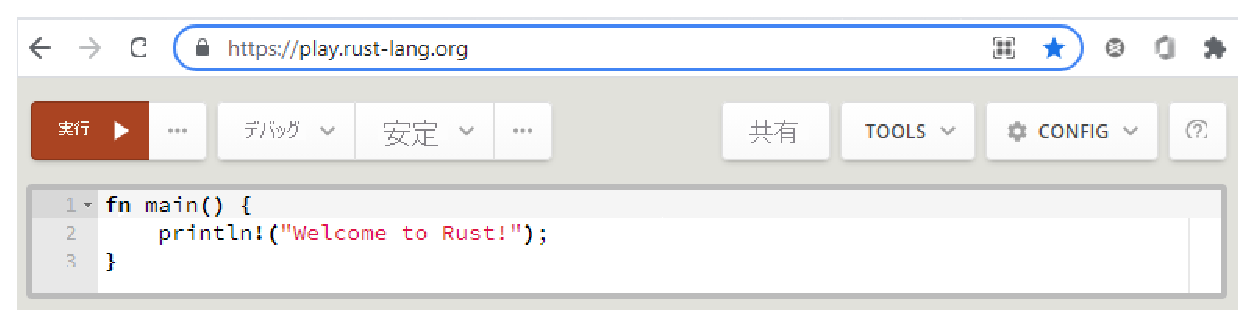
\includegraphics[width=14cm]{rust-playground-main.eps}

プレイグラウンドでは、Rust \texttt{std} 標準ライブラリのメソッドと関数にアクセスできます。 crates.io ライブラリで最もダウンロードされている上位 100 のクレートも、それらの依存関係と共に使用できます。

\subsubsection{ツールと機能}

Rust プレイグラウンドには、組み込みのツールと開発機能がいくつか用意されています。

\begin{itemize}
\item 書式コード: Rustfmt ツールを使用すると、公式の Rust スタイルを使用するようにコードを書式設定できます。 このツールによってコードが調整され、要素と演算子の間に推奨されているインデントと間隔が適用されます。
\item テスト コード: Clippy ツールでは、コード内に誤りがないかどうか確認します。 このツールでは、コードに対して lint テストを実行し、エラーや改善する領域を見つけることができます。
\item コードの保存: Rust プレイグラウンドでの作業時に、そのコードがブラウザーのローカル ストレージに自動的に保存されます。 この機能により、特にブラウザー ウィンドウを偶然閉じてしまった場合に、最新の作業を簡単に復旧できます。
\item コードの共有: [共有] 機能により、プレイグラウンド内のコード用に共有可能な GitHub gist が作成されます。 この URL を保存することで、後でコードにアクセスできます。 URL によって、特定のコードの gist がプレイグラウンドに読み込まれます。
\end{itemize}

\begin{itembox}[l]{注意}
ブラウザーのローカル ストレージは、シングルトン リソースです。 複数のブラウザー ウィンドウで Rust プレイグラウンドを開き、各ウィンドウで異なるコードを操作している場合、すべてのウィンドウの中で最後に保存されたコードだけがローカル ストレージに保持されます。
\end{itembox}

\subsubsection{ビルド オプション}

Rust プレイグラウンドには、コードをビルドして実行するためのいくつかのオプションがあります。

\begin{itemize}
\item \textbf{Run}: コードをビルドして実行し、出力を表示します。 [Run] オプションは、 コマンドを使用することと同じです。
\item \textbf{Build}: コードをビルドしますが、そのコードは実行しません。 [Build] オプションは、 コマンドを使用することと同じです。
\item \textbf{Test}: コードをビルドし、そのコードに対してすべてのテストを実行します。 [Test] オプションは、 コマンドを使用することと同じです。
\end{itemize}

\subsubsection{保護の制限}

プレイグラウンドには、サイトが不正な手段で使用されるのを防ぐ制限事項が設けられています。 この制限事項により、すべてのユーザーがこのサイトを使用し続けることができます。

\begin{itemize}
\item \textbf{ネットワーク}: プレイグラウンドでコードをコンパイルまたは実行するときは、ネットワーク接続を使用できません。
\item \textbf{メモリ}: プレイグラウンドでは、コードをコンパイルしてビルドされたプログラムを実行するために使用できるメモリが制限されます。
\item \textbf{実行時間}: プレイグラウンドでは、コードをコンパイルしてビルドされたプログラムを実行する最大時間が設定されています。
\item \textbf{ディスク}: コードをコンパイルしてビルドされたプログラムを実行するために使用できるディスク領域の量は制限されています。
\end{itemize}



Rust プレイグラウンドの機能の詳細については、Rust の Web サイトを参照してください。


\subsubsection{自分の知識をチェックする}

次の質問に答えて、学習した内容を確認してください。

\begin{enumerate}
\item コードの間違いを見つけるために使用できる Rust プレイグラウンド ツールはどれですか?
\begin{itemize}
\item rustfmt
\item Clippy
\item デバッグ
\end{itemize}
\item Rust プレイグラウンドでネットワーク接続を利用できなくなるのはどのようなときですか。
\begin{itemize}
\item コードの編集中。
\item プログラムの実行中。
\item コードのコンパイル中、またはプログラムの実行中。
\end{itemize}

\end{enumerate}


